\section{Simulation Analysis}
\label{sec:simulation}

\paragraph{}
In this section, we can find the results of each topic required in the simulation analysis. The numeric results or graphics are presented alongside a short explanation of the interpretation of the problem. All of the results were obatined usig NGSpice and the section is dividid in five different subsections - Subsection ~\ref{subsec:sim_first}, Subsection ~\ref{subsec:sim_second}, Subsection ~\ref{subsec:sim_third}, Subsection ~\ref{subsec:sim_fourth} and Subsection ~\ref{subsec:sim_fifth}, one for each topic of the simulation analysis.

\paragraph{}
Ngspice is a circuit-simulation program that makes it possible to have an accurate representation of how the circuit would behave if it was actually assembled. The different tables shown below ilustrate the simulated operating point results for the circuit under analysis. As it can be seen, the tables show the values of the voltage in all nodes, the currents in all of the branches and also the currents in independent voltage sources.

\paragraph{}
Sometimes, when looking at the simulation results there is one very interesting detail which is very important: Ngspice operates with the idea that the positive current flows from the positive pole to the negative pole in all components, sources included. This explains why, in some cases, in the the very same branch where a voltage source is located, the current given by Ngspice in the whole branch is the symetric of the one given specifically in the voltage source. Another important detail about this operating point analysis of the circuit is thta the node $n_A$ and the voltage source $V_{AB} = 0V$, which are absent from the circuit’s picture. This is because the Current-Controlled Voltage Source is dependent on current $I_D$ , but Ngspice requires a voltage source where this current flows through, which made necessary the use of an auxiliary voltage source in series with $R_6$ and, therefore, an auxiliary node.


\subsection{Simulation - Topic I}
\label{subsec:sim_first}

\begin{table}[H] \centering
  \begin{tabular}{|l|r|}
    \hline    
    {\bf Node/Component} & {\bf Value [A or V]} \\ \hline
    \input{op1_TAB}
  \end{tabular}
  \caption*{Voltages and the currents in all nodes and in all branches}
 \label{tab:op1}
\end{table}

\paragraph{}
For topic 1 of the simulation analysis section, we can see, in this table, the results of the simulation used to determine the voltages and the currents in all nodes and in all branches, respectively, by simulating the operating point for $t<0$.
%%%%%%%%%%%%%%%%%%%%%%%%%%%%%%%%%%%%%%%%%%%%%%%

\subsection{Simulation - Topic II}
\label{subsec:sim_second}

\begin{table}[H] \centering
  \begin{tabular}{|l|r|}
    \hline    
    {\bf Node/Component} & {\bf Value [A or V]} \\ \hline
    \input{op2_TAB}
  \end{tabular}
  \caption*{Voltages and currents obtained by simulating the operating point for $vs(0)=0$ and replacing the capacitor with a voltage source}
 \label{tab:op1}
\end{table}

\paragraph{}
For topic 2, by simulating the operating point for $vs(0)=0$, and replacing the capacitor with a voltage source $Vx = V(6)-V(8)$, where V(6) and V(8) are the voltages in nodes 6 and 8 as obtained in topic 1, we obtain the results printed in tabel above. We do this step in order to use Thevenin´s Theorem to simplify this complex circuit, turning it into a more simple equivalent circuit consisting of a resistance in series with a source voltage.
%%%%%%%%%%%%%%%%%%%%%%%%%%%%%%%%%%%%%%%%%%%%%%%

\subsection{Simulation - Topic III}
\label{subsec:sim_third}

\begin{figure}[H] \centering
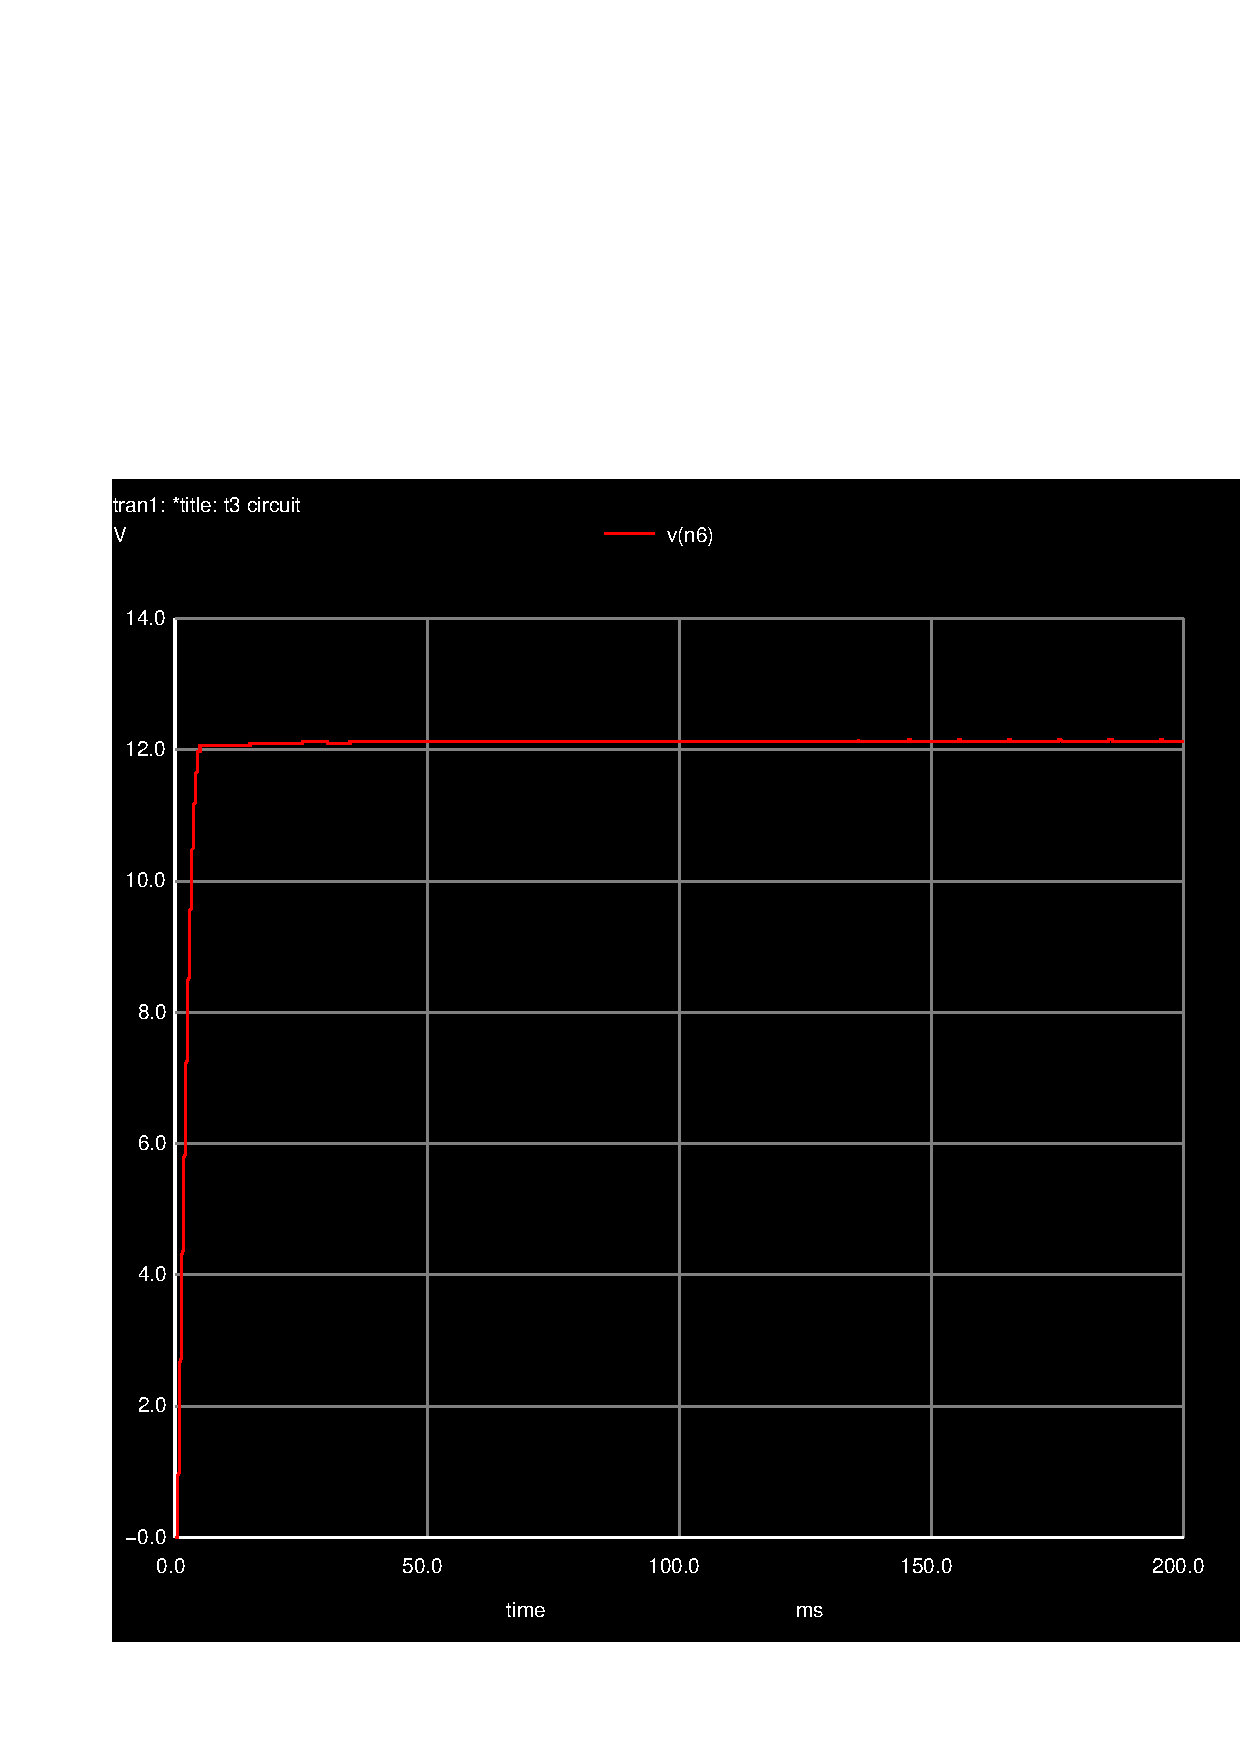
\includegraphics[width=0.4\textwidth]{trans1.pdf}
\caption{Natural response of the circuit.}
\label{fig:natural}
\end{figure}

\paragraph{}
For topic 3, by using the boundary conditions V(6) and V(8) obtained in topic 2, and by using Ngspice’s transient analysis mode to get v6(t) in the interval [0, 20] ms, we can simulate the natural response of the circuit and plot the results, as presented in the figure above.

%%%%%%%%%%%%%%%%%%%%%%%%%%%%%%%%%%%%%%%%%%%%%%%

\subsection{Simulation - Topic IV}
\label{subsec:sim_fourth}

\begin{figure}[H] \centering
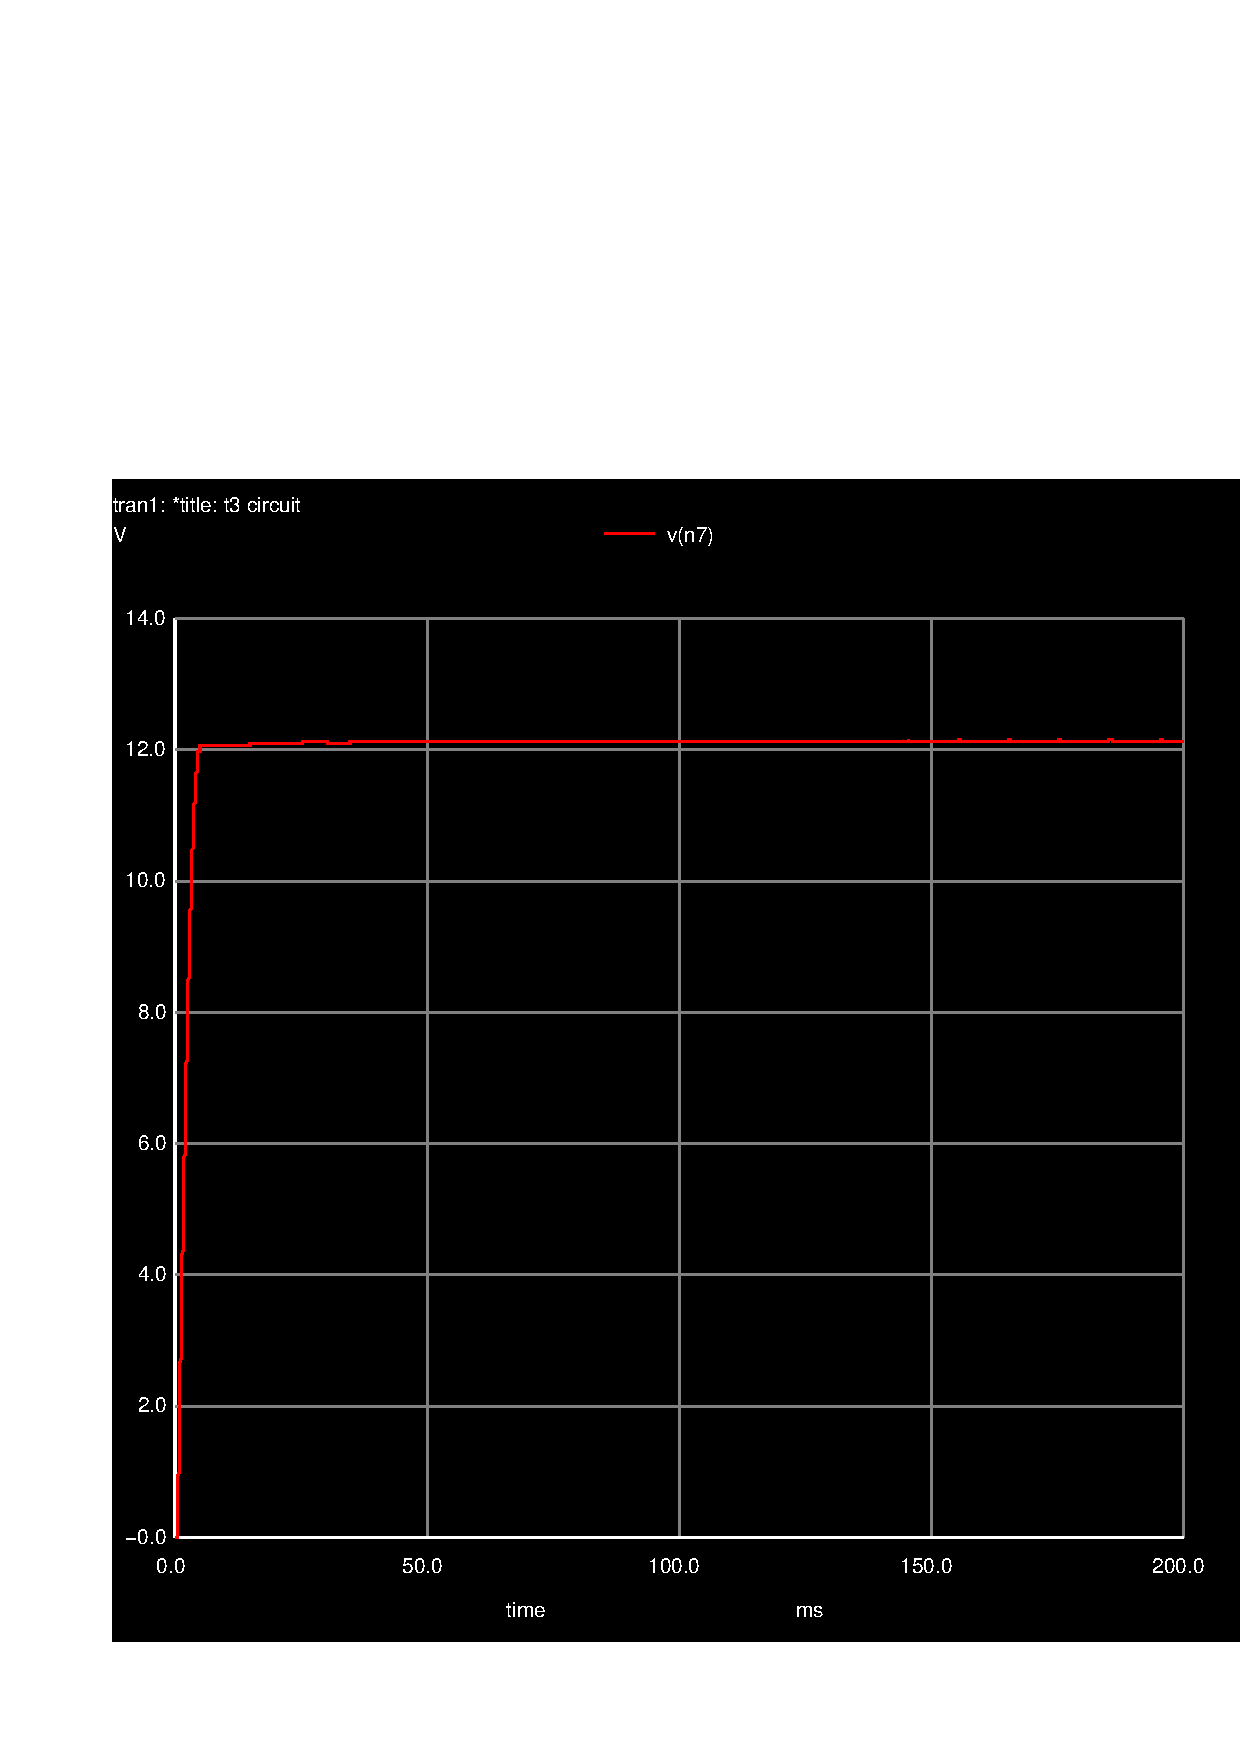
\includegraphics[width=0.4\textwidth]{trans2.pdf}
\caption{Total response of the circuit.}
\label{fig:total}
\end{figure}

\paragraph{}
Regarding topic 4, the above figure is ploted by simulating the total response on node 6, that is, the natural and the forced solutions, by repeating the step presented in topic 3 with $v_s(t) = V_s u(-t) + sin(2 \pi ft) u(t)$ and frequency equal to 1 $KH_z$. 

%%%%%%%%%%%%%%%%%%%%%%%%%%%%%%%%%%%%%%%%%%%%%%%%%%

\subsection{Simulation - Topic V}
\label{subsec:sim_fifth}

\begin{figure}[H] \centering
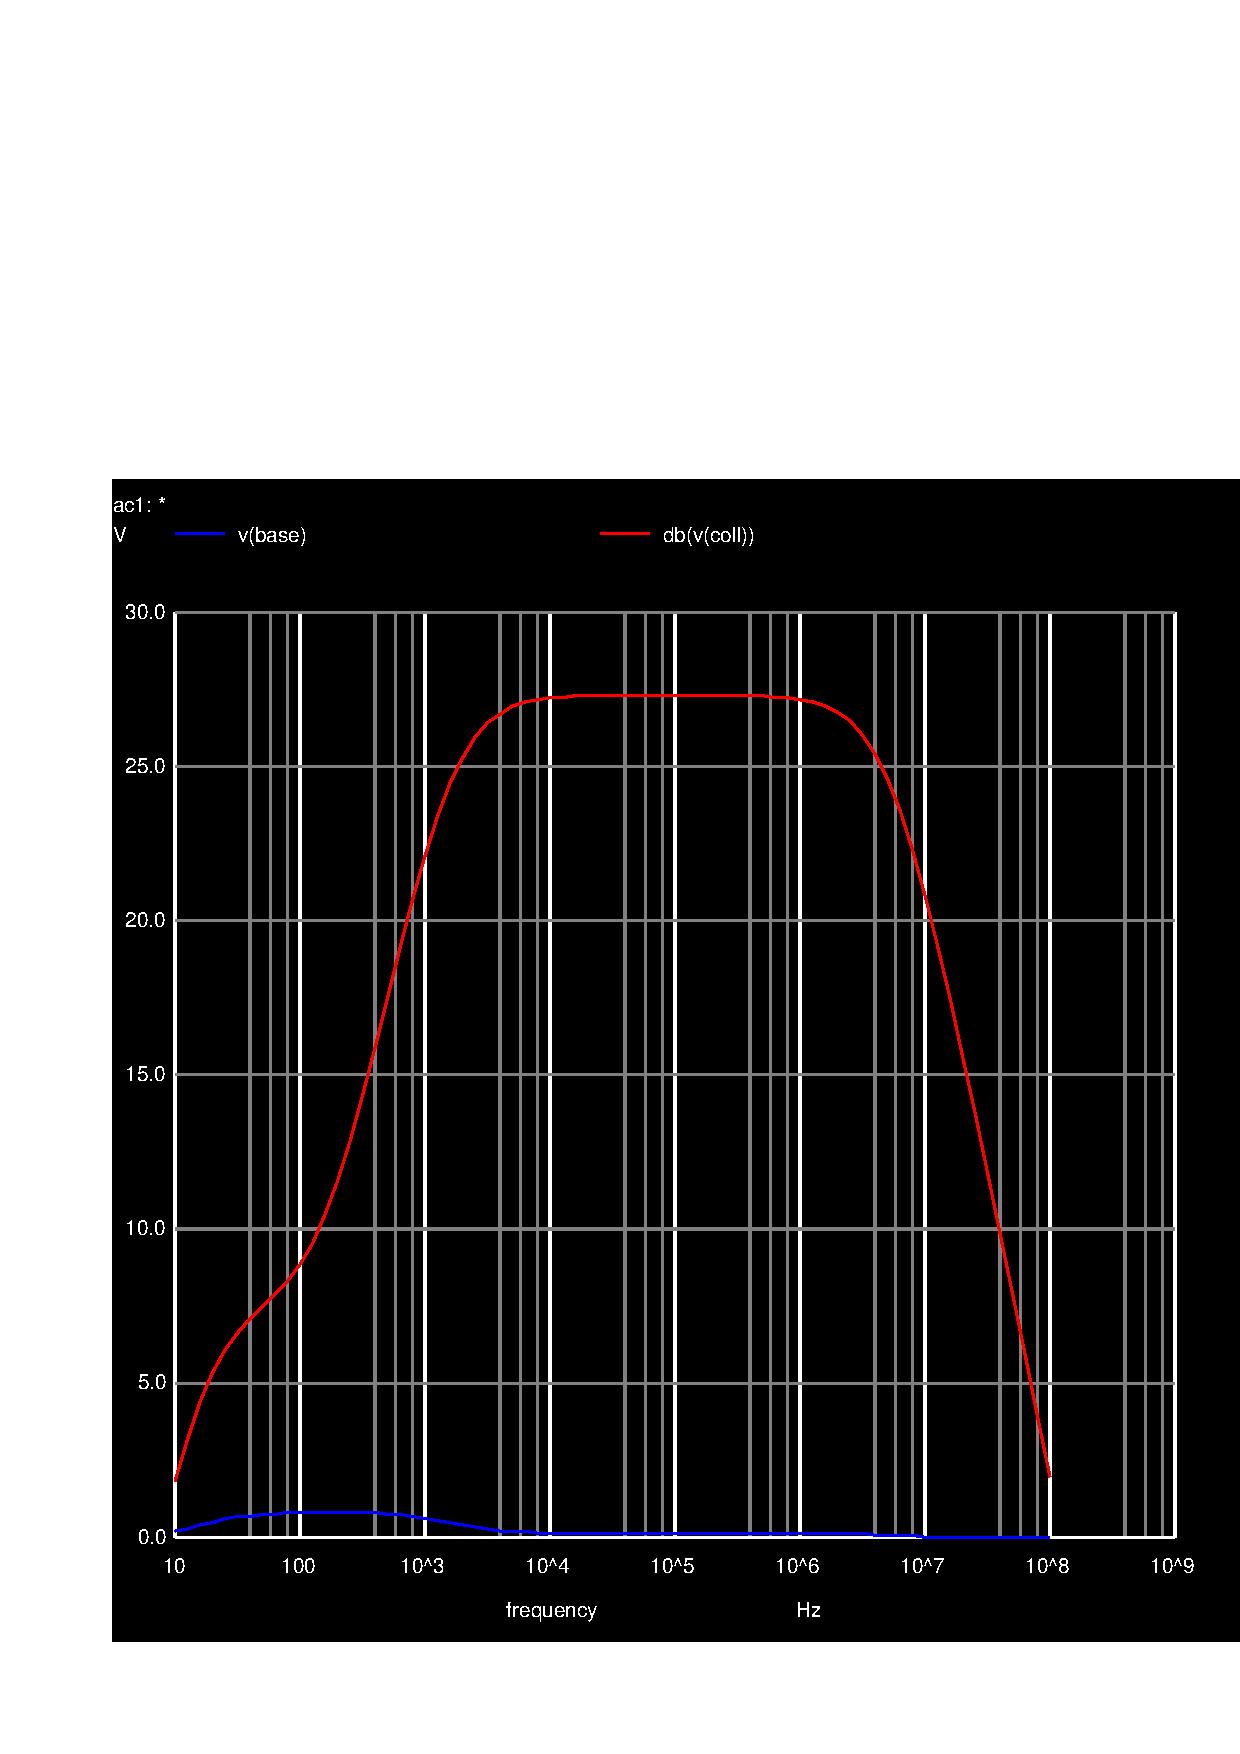
\includegraphics[width=0.4\textwidth]{acm.pdf}
\caption{Magnitude of $v_s(f)$ and $v_6(f)$ during frequency interval [0.1 , 1] MHz.}
\label{fig:$V_s(f)$}
\end{figure}


\begin{figure}[H] \centering
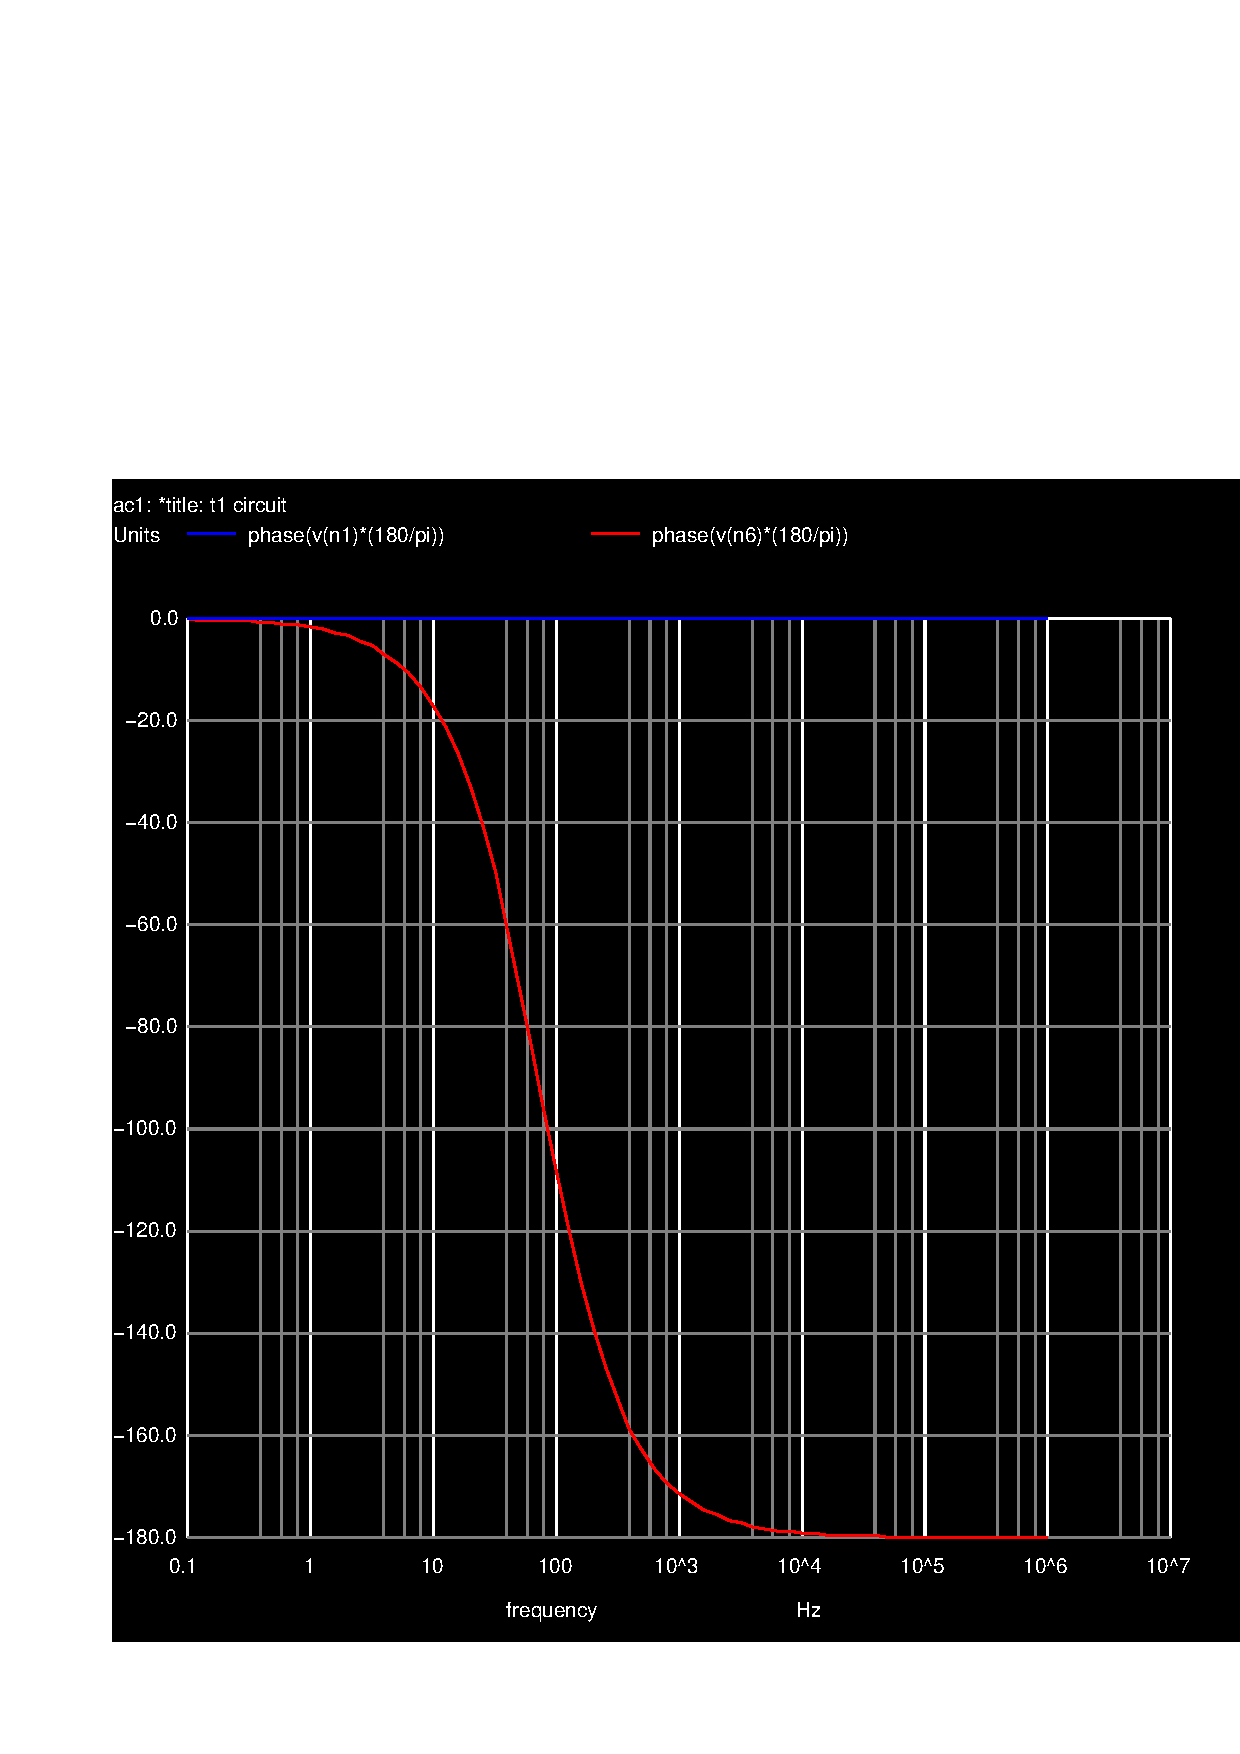
\includegraphics[width=0.4\textwidth]{acp.pdf}
\caption{Phase of $v_s(f)$ and $v_6(f)$ during frequency interval [0.1 , 1] MHz.}
\label{fig:$V_6(f)$}
\end{figure}

\paragraph{}
Furthermore, in topic 5, we simulate the frequency response in node 6 (it is important to note that the frequency is presented in a logarithmic scale, the magnitude in dB and the phase in degrees) for the frequency range of 0.1 Hz to 1 MHz. Finally, we plot both vs(f) and v6(f), as presented in the figures above. The differences between the magnitude and phase of the two voltages are explained because they correspond to different nodes.

\paragraph{}
By analysing both the plots, we can conclude that the function that describe each one of the node voltages are, in fact, similar in the representation of its magnitude and phase. As it can be seen, the magnitude of $v_s$ is null and it remains constant till the end of the time interval. The magnitude of node voltage $V_6$ is represented by a curve that shows variation through frequency. This magnitude is described by a descent of the node voltage values, which start with a constant value around 1 db and tends to stabilize near -5 db in the final section of the interval. As previously stated for the magnitude, also the phase of $v_s$ is null and remains constant till the end of the time interval. On the other hand, the phase of node voltage $V_6$ is also null in the beggining of the time interval. However, as we can see, the phase of this node voltage is represented by a curve that shows a descent variation through time. This phase can be described by this curve with an inflexion point in the middle value of the time interval that tends to stabilize near -100 degrees.

